% LaTeX layout by Jonas Kahler, jonas@derkahler.de
% HashTux SAD Document
% Group Tux:
% Aman Dirar, Jerker Ersare, Jonas Kahler, Dennis Karlberg
% Niklas le Comte, Marco Trifance, Ivo Vryashkov
% Chapter 3 - Resulting Architecture Overview
\chapter[Resulting Architecture Overview]{Resulting Architecture\\ Overview}
We received clear recommendations from our supervisor and others to not use
Erlang for serving web pages. Therefore we decided to use a common web server
for hosting the web content, and PHP as our (web) server side language. Our
solution consists of the Client UI, two server side components, and we also use
the CouchDB DBMS.
\begin{itemize}
  \item Client UI, rendered in a web browser, uses JavaScript
  \item PHP application, executed on an Apache web server
  \item Backend server, written in Erlang, connecting to CouchDB and social
     media APIs
  \item CouchDB Database (External component)
\end{itemize}
Our application can be said to use the layered architectural style. Each layer
can use the services provided by the layer below. The modules in JavaScript and
PHP can be said to make up the UI Layer, while the Erlang code is used both for
the Application Layer and the Data Layer. \newline

\begin{figure}[ht]
  \centering
  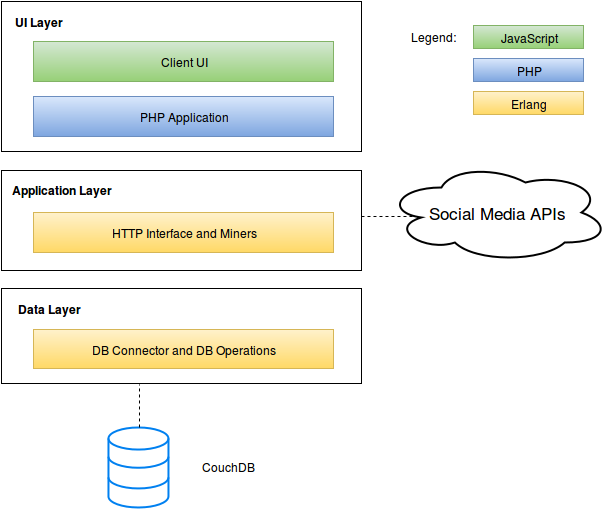
\includegraphics[width=0.8\textwidth]{hashtux_layers.png}
  \caption{HashTux Layer Diagram}
\end{figure}